\chapter{Grundlagen}
In diesem Kapitel werden einige Grundlagen erläutert, die für den weiteren Verlauf der Arbeit relevant sind.

\section{(Präklinische-) Magnetresonanztomographie}
Magnetresonanztomographie (abgekürzt MRT\footnote{Auch \textit{MRI} (englisch magnetic resonance imaging)}) bezeichnet ein bildgebendes Verfahren, dass den physikalischen Effekt der Kernspinresonanz (NMR nach englisch nuclear magnetic resonance) nutzt.

Als \textit{Tomografie}\footnote{von altgriechisch tome, Schnitt und graphein, schreiben}-Verfahren ermöglicht es MRT, dreidimensionale Strukturen als Schnittbilder aufzunehmen und wieder in 3D darzustellen. Die Schnittbilder geben die innere Struktur eines Objektes dabei so wieder, als wäre das Objekt tatsächlich in der betrachteten Ebene geschnitten. Insbesondere sind die Bilder im Vergleich zu Projektionsverfahren (wie z.B. der klassischen Röntgenaufnahme) überlagerungsfrei.

Im Gegensatz zur \textit{Computertomographie} (CT), einem weiteren sehr verbreitetem Tomographieverfahren, kommt bei einer MRT Untersuchung keine ionisierende Strahlung zum Einsatz.

Die folgenden Abschnitte beschreiben den NMR-Effekt und die weiteren Techniken, die zur Bildentstehung in einem MRT Gerät nötig sind. Im letzten Abschnitt wird auf die Besonderheiten der präklinischen Bildgebung eingegangen.

\subsection{Der NMR-Effekt}
Die Entwicklung der Magnetresonanzbildgebung wurde erst durch die Entdeckung der Kernspinresonanz möglich. Der physikalische Effekt wird auch außerhalb englischsprachiger Länder meist \textit{nuclear magnetic resonance}, kurz NMR, genannt.

\subsubsection{Geschichte}
1922 zeigten \textsc{Stern} und \textsc{Gerlach} im, nach ihnen benannten, Stern-Gerlach-Experiment die Quantelung von (Eigen-) Drehimpulsen: Silberatome werden aus einem Ofen heraus durch ein inhomogenes Magnetfeld auf eine Glasplatte beschleunigt. Klassisch wäre durch die Ablenkung des Magnetfeldes eine kontinuierliche Intensitäts-Verteilung um $0\degree$ auf der Platte zu erwarten. Stattdessen entstehen durch die quantisierten Spins zwei diskrete Punkte. \cite{Gerlach1922}

1938 konnte die Kernspinresonanz erstmals von \textsc{Isidor Isaac Rabi} durch eine Erweiterung des Stern-Gerlach-Versuchs nachgewiesen werden: Dazu wird die Anordnung des Stern-Gerlach-Versuchs um ein weiteres inhomogenes Magnetfeld dahinter ergänzt. Dieses ist umgekehrt gepolt und ansonsten identisch dem ersten Feld. Das erste Feld wirkt daher de-fokussierend auf die Atome, das zweite re-fokussierend. Wird ein homogenes Wechsel-Magnetfeld zwischen den beiden inhomogenen Feldern erzeugt, sinkt die gemessene Detektorintensität hinter der Anordnung bei einer bestimmten Frequenz. Bei dieser Frequenz $\omega_0$ wird die Resonanzbedingungen zwischen zwei Übergängen erreicht. $\omega_0$ heißt daher Resonanzfrequenz. Damit ist es möglich, die benötigte Energie zu bestimmen, um ein atomares, magnetisches Moment anzuregen. Für seine Arbeiten erhielt Rabi 1944 den Nobelpreis für Physik. \cite{Rabi1938}

Weitere Pionierarbeit auf dem Gebiet der NMR leisteten der Schweizer Physiker \textsc{Felix Bloch} und der US-Amerikaner \textsc{Edward Mills Purcell}: Mit unterschiedlichen Versuchsaufbauten entdeckten die Physiker in den 1940er Jahren fast zeitgleich und unabhängig voneinander die NMR in Flüssigkeiten bzw. Feststoffen. Bloch und Purcell wurde 1952 gemeinsam der Nobelpreis für Physik verliehen.

\todoin[]{Lautabur etc.}

\subsubsection{Quantenmechanische Theorie}

\begin{equation}
	\omega_0=\gamma B_0
\end{equation}
mit:
\begin{with}
\omega_0 & Kreisfrequenz (in \SI{}{\hertz}) \\
\end{with}

\subsubsection{Blochgleichungen}
Die Blochgleichungen gelten in Flüssigkeiten und eingeschränkt auch in Festkörpern. In vektorieller Schreibweise lauten sie:
\begin{equation}
	\frac{d\vec{M}}{dt}=\gamma\vec{M}\times\vec{H_a}-\vec{e_x}\frac{M_x}{T_2}-\vec{e_y}\frac{M_y}{T_2}-\vec{e_z}\frac{M_z-M_0}{T_1}
\end{equation}
mit:
\begin{with*}
	\vec{M} & Magnetisierung \\
	T_1,T_2 & Relaxationszeiten \\
\end{with*}

\todoin{Unterschied Laborsystem, rotierendes Bezugssystem}


\subsubsection{Relaxation}
\todoin[]{T1, T2, pD gewichtung}

\subsection{Kernspin detektierbare Eigenschaften von Gewebe}
Als bildgebendes Verfahren ist es das Ziel eines Tomographen Gewebe zu identifizieren und von benachbartem Gewebe zu unterscheiden. Um also zwei Gewebearten in einem MRT Schnittbild unterscheiden zu können, ist es notwendig, dass sich die Gewebe in ihren NMR Eigenschaften hinreichend unterscheiden und, dass dieser Unterschied auch vom Gerät erfasst werden kann. Ein Vergleich einiger Gewebearten zeigt \autoref{tab:gewebe}. Es wird deutlich, dass sich beispielsweise eine Metastase in der Leber mit einer T1 gewichteten MRT Aufnahme gut nachweisen lässt, da sich die T1 Zeiten von gesundem Lebergewebe und der Metastase deutlich unterscheiden.

\begin{table}[H]
	\centering
	\caption[MRT relevante Eigenschaften ausgewählter Gewebe]{MRT relevante Eigenschaften von einigen ausgewählten Gewebearten bei einer Feldstärke von \SI{1.5}{\tesla} (in Anlehnung an \cite[S.~16]{Weishaupt2014} und \cite[S.~17]{Reiser2008})}
	\label{tab:gewebe}
	\begin{tabular}{llll}
		\toprule
		\textbf{Gewebe} & \textbf{Protonendichte (in \%)} & \textbf{T1 (in ms)} & \textbf{T2 (in ms)} \\
		\midrule
		Zerebrospinalflüssigkeit & 100 & \textgreater4000 & 2000 \\
		weiße Hirnsubstanz & 70 & 780 & 90 \\
		graue Hirnsubstanz & 85 & 920 & 100 \\
		Fettgewebe & 100 & 260 & 80 \\
		Leber & - & 500 & 43 \\
		Niere & - & 650 & 58 \\
		Metastase & 85 & 1800 & 85 \\
		\bottomrule
	\end{tabular}
\end{table}

\autoref{fig:metastase} zeigt ein T1 gewichtetes, axiales Schnittbild durch eine von Darmkrebs verursachte Metastasierung in der Leber. Das umliegende gesunde Gewebe kann deutlich von den Metastasen abgegrenzt werden.

\begin{figure}[H]
	\centering
	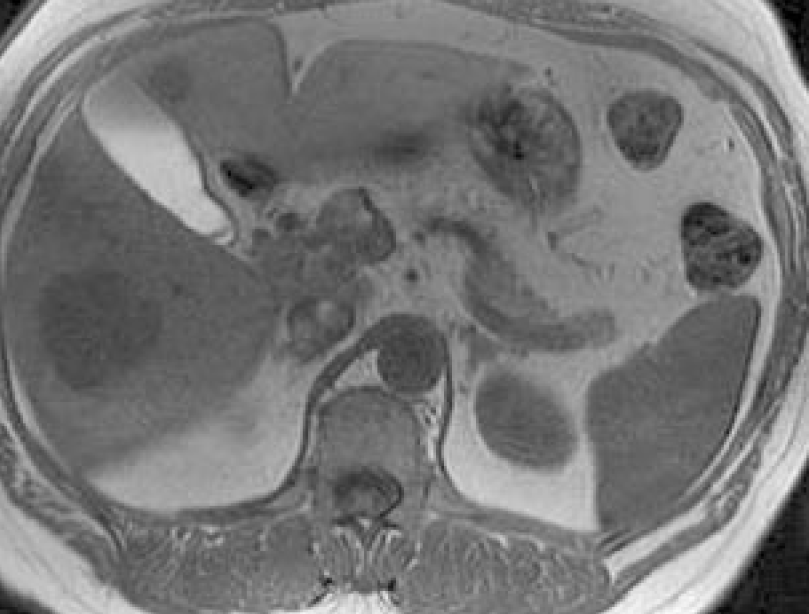
\includegraphics[width=0.5\textwidth]{img/metastase.png}
	\caption[Lebermetastase]{Lebermetastase. Axialer Schnitt, T1 gewichtete spoiled gradient Aufnahme mit Fettunterdrückung, kein Kontrastmittel \cite[S.~872]{Reiser2008}}
	\label{fig:metastase}
\end{figure}



\subsection{Aufbau eines MR-Tomographen}
\missingfigure{Gesamtsystem}

\subsubsection{Statisches Magnetfeld}
Das statische Magnetfeld, auch $B_0$-Feld genannt, wird durch einen Magneten erzeugt. Dieser muss über eine ausreichend dimensionierte Öffnung verfügen, so dass der zu untersuchende Körper und andere Spulensysteme des Tomographen darin Platz finden. Mit Feldstärken im Bereich von \SI{0.3}{\tesla} (bei klinischen MRI Systemen) bis hin zu \SI{15}{\tesla} im Bereich der präklinschen MRIs ist das $B_0$-Feld verglichen mit dem Erdmagnetfeld\footnote{etwa \SI{50}{\micro\tesla} \cite{Enc1994}} oder einem Kühlschrankmagneten\footnote{etwa \SI{0.1}{\tesla} \cite{LHC2018}} ein sehr starkes Magnetfeld.
Erzeugt wird das $B_0$-Feld entweder mit einem Permanentmagneten oder einem Elektromagneten. 

Auch wenn sich \textit{Permanentmagnet}systeme durch ihren einfachen Aufbau und einen kostengünstigen, wartungsfreien Betrieb auszeichnen, sind sie wenig stark verbreitet. Die mit Permanentmagneten erzielbare Feldstärke von etwa einem Tesla ist für Forderung nach hohen Signal-Rausch-Verhältnissen oft zu gering.

Gewöhnliche Elektromagnete, auch \textit{resistive Elektromagnete} genannt, haben den Nachteil des hohen Stromverbrauchs und der starken Eigenerwärmung. Von Vorteil ist, dass Systeme dieser Bauart bei Nicht-benutzen abgeschaltet werden können. Für sehr hohe Feldstärken sind sie nicht geeignet.

Am weitesten verbreitet sind \textit{supraleitende Elektromagnete}. Nur damit lassen sich wirtschaftlich hohe Feldstärken erreichen. Diese bestehen aus einer supraleitenden Spulenanordnung, welche in einem, mit flüssigem Helium gefülltem, Tank betrieben wird. Da aufgrund der Supraleitung der Spulenwiderstand verschwindet, kann nach einmaligem Aufbau des Spulenstroms die Stromversorgung getrennt werden. Das als Kryostat bezeichnete Kühlsystem verliert durch den sog. \textit{boil-off} kontinuierlich Helium, welches daher regelmäßig wieder aufgefüllt werden muss. Ein Abschalten der Engergie- und Kosten-intensiven Kühlung ist nicht möglich. Eine Erwärmung der ganzen Spule, oder Teile davon über die Sprungtemperatur des Spulenmaterials führt zum sog. \textit{Quench}: Die Supraleitung bricht zusammen, das Material wird resistiv und durch die damit verbundene starke Wärmeentwicklung verdampft das gesamte Helium schlagartig. Daher ist es nötig, dass das Kryostat über einen Kamin zur Ableitung des Heliums verfügt. Wenn auch für den Menschen ungiftig, können größere Mengen Helium den Luftsauerstoff verdrängen. Daher muss die Sauerstoffkonzentration in den Aufstellungsräumen überwacht werden.

\todoin{Zylinder vs platten}

\paragraph{Shimming}\mbox{}\\
An das statische Magnetfeld werden hohe Anforderungen bezüglich der Feldhomogenität gestellt.
Durch Metalle im Tomographen (Rohre, Schrauben, Befestigungen, etc.) und am Aufstellungsort (z.B. Stahlträger/Metallständerwände), Streufelder anderer Magnete und in die Nähe des Tomographen gebrachte Metalle kommt es zu Inhomogenitäten.
Um diese auszugleichen, wird Shimming (von eng. \textit{shim}, Keil) betrieben. Unterschieden werden passives und aktives Shimming \cite{Lipton2008}:
\begin{itemize}
	\item \textbf{passives Shimming:} Durch gezieltes Einbringen von ferromagnetichen Metallen\footnote{z.B. Eisen oder Nickel} werden Inhomogenitäten statisch korrigiert. Damit können lediglich intrinsische Effekte des MRT-Systems und des Gebäudes ausgeglichen werden.
	\item \textbf{aktives Shimming:} Durch zusätzliche Spulen\footnote{meist in resistiver Ausführung} werden (schwache) Korrektur-Felder erzeugt. Der Vorteil hierbei ist, dass dynamisch korrigiert werden kann: Kurz vor einer MRT Aufnahme kann das aktive Shimming genutzt werden, um Inhomogenitäten  durch die Probe zu mindern.  
\end{itemize}

\subsubsection{Gradientenspulen}
Das Gradientensystem besteht aus mehreren Spulenanordnungen, die dem starken statischen Feld schwächere, zeitlich variable Felder überlagern. Im Gegensatz zum $B_0$-Feld, sind diese Felder \textit{in}homogen. Ihre Feldstärke variiert linear mit dem Ort. Diese lineare Feldänderung wird als Gradient bezeichnet und ist meist in x, y und z-Richtung ausgeprägt. Da diese Felder schnell umgeschaltet werden müssen, können sie nicht als supraleitende Spulen ausgeprägt werden, sondern sind resistiver Art. Das schnelle Umschalten erfordert leistungsstarke elektrische Verstärker.


\subsubsection{RF Sende- und Empfangsspulen}
Das Hochfrequenzsignal wird über die RF Spulen eingestrahlt. Entweder über die gleiche Spule, oder über separate Empfangsspulen wird das entstehende MR-Signal empfangen.

\subsubsection{Abschirmung}
Zum Schutz des MRT vor externer Störstrahlung und zum Schutz der Umgebung (Menschen und andere Geräte) sind Abschirmungen nötig:
Das Magnet für das statische Magnetfeld erzeugt nicht nur das nutzbare $B_0$-Feld, sondern auch magnetische Streufelder. Diese können passiv, z.B, durch Stahlplatten, oder aktiv durch zusätzliche Spulen abgeschirmt werden.

Von den Gradientenspulen erzeugte Streufelder, welche durch Wirbelströme entstehen, können auf ähnliche Art und Weise unterdrückt werden.

Eine RF-Abschirmung des Raumes, in dem der MR-Tomograph betrieben wird, ist notwendig, damit das MRT Gerät keine Störstrahlung nach Außen emittiert und damit keine externen Störsignale die Bildaufnahme stören können.
Dazu ist es zum Beispiel möglich, den kompletten Raum mit einem Metall auszukleiden, um einen Faradayschen Käfig zu bilden. Kupfer ist dafür gut geeignet, da aufgrund seiner geringen Skin-Tiefe im Megahertz-Bereich eine dünne Folie ausreichend ist. \cite{Weibler1993} Problematisch ist die ausreichende Abschirmung der Eingangtür. Durch Materialverschleiß treten dort besonders häufig RF-Lecks auf.


\subsection{Bildentstehung im MR-Tomographen}

\subsubsection{Selektive Anregung/Schichtwahl}
Zur Auswahl einer Schicht parallel zur z-Ebene wird während der Einstrahlung des HF-Pulses ein Gradient in z-Richtung, $G_z=\frac{\partial B_z}{\partial z}$ eingeschaltet.

Die Amplitudenfunktion $B_T(t)$ mit der das HF-Signal moduliert wird, wird so gewählt, dass eine möglichst scharf begrenzte Schicht in z-Richtung selektiert wird.

\begin{figure}[H]
	\centering
	\resizebox{!}{!}{\includegraphics[]{img/rfForm.tikz}}
	\caption[form]{HF puls}
	\label{fig:rfForm}
\end{figure}

Daher wird meist
\begin{equation}
	B_T(t)=C \frac{sin(x)}{x}
\end{equation}
als Amplitudenfunktion gewählt, da...


\subsubsection{Phasenkodierung}

\subsubsection{Frequenzkodierung}

\subsection{MRT Pulssequenzen}
Die zeitliche Abfolge der Gradientenfelder (Schichtwahl, Phasenkodierung und Frequenzkodierung) und der Hochfrequenz-Anregungssignale wird als MRT Pulssequenz bezeichnet.
Drei wichtige, so genannte Basispulssequenzen sind \cite[S. 999]{Weishaupt2014}:
\begin{itemize}
	\item \textbf{SE}: Spinecho-Sequenz
	\item \textbf{IR}: Inversion-Recovery-Sequenz
	\item \textbf{GRE}: Gradientenecho-Sequenz
\end{itemize}

Darüber hinaus gibt es heute zahlreiche weitere Sequenzen, die zum Beispiel für spezielle Aufnahme-Modi, wie die Diffusionsbildgebung nötig sind oder die Aufnahmezeit stark verkürzen. Zwei Beispiele für die "schnellen" Sequenzen sind \textit{Turbo-Spinecho} und \textit{Echo Planar Imaging}.


\subsubsection{Spinecho-Sequenz}
Bei der Spinecho-Sequenz, abgekürzt mit \textit{SE}, erfolgt zunächst eine Anregung der Schicht mit einem 90\degree-RF-Puls, der die Spins in die XY-Ebene klappt. Durch statische Feldinhomogenitäten im Gewebe zerfällt die Magnetisierung nicht mit T2, sondern mit T2*. Da die Spins auseinanderlaufen, wird dieser Prozess als Dephasierung bezeichnet. Nach der Hälfte der Echozeit ($TE/2$) wird ein 180\degree-RF-Puls eingestrahlt. Dieser klappt das Spin-Ensemble um 180\degree. Die Spins laufen daraufhin nach der Zeit $2(TE/2) = TE$ wieder zusammen; es kommt zur Rephasierung. Das dabei entstehende Empfangssignal wird \textit{Echo} genannt (\autoref{fig:SE}).

Nach der Repetitionszeit $TR$ wird die Sequenz wiederholt. Durch Variation des Phasenkodiergradienten $G_{ph}$ wird bei jeder Wiederholung eine andere Zeile des k-Raums ausgewählt, die dann mit dem Frequenzkodiergradienten $G_f$ Pixelweise ausgelesen wird.

Die SE-Sequenz hat den Vorteil, dass statische Feldinhomogenitäten vollständig ausgeglichen werden. Durch die einstellbaren Zeiten $TE$ und $TR$ kann eine T1, T2 oder PD gewichtete Aufnahme erzeugt werden.
Der sehr guten Bildqualität steht die lange Aufnahmezeit gegenüber.

\begin{figure}[H]
	\centering
	\resizebox{!}{!}{\includegraphics[]{img/SE.tikz}}
	\caption[Spinecho-Sequenz]{Zeitverlauf der Signale im MRT bei einer Spinecho-Sequenz}
	\label{fig:SE}
\end{figure}

\subsubsection{Inversion-Recovery-Sequenz}
Eine Variation der Spinecho-Sequenz ist die Inversion-Recovery-Sequenz, kurz IR-Sequenz. Dabei wird vor dem 90\degree-RF-Anregungspuls ein 180\degree-RF-Puls eingestrahlt. Die Zeit zwischen dem 180\degree-RF-Puls (dem sog. Inversionspuls) und dem Anregungspuls wird als Inversionszeit $TI$ (time of inversion) bezeichnet. Durch die einstellbare Inversionszeit kann das Signal einiger Gewebetypen unterdrückt werden oder es können stark T1 gewichtete Bilder erzeugt werden (\autoref{fig:IR}).

\begin{figure}[H]
	\centering
	\resizebox{!}{!}{\includegraphics[]{img/IRE.tikz}}
	\caption[Inversion-Recovery-Sequenz]{Zeitverlauf der Signale im MRT bei einer Inversion-Recovery-Sequenz}
	\label{fig:IR}
\end{figure}

\subsubsection{Gradientenecho-Sequenz}
Bei der Gradientenecho-Sequenz (GRE) wird kein 180\degree-RF-Puls zur Erzeugung eines Echos, sondern ein Polaritätswechsel des Frequenzkodiergradientens genutzt. Dadurch, dass der 180\degree-Puls eingespart werden kann, sind viel kürzere Repetitionszeiten $TR$ möglich. Da bei einer kleinen Repetitionszeit auch nur wenig Zeit für eine vollständige T1-Relaxation zur Verfügung steht, werden häufig Anregungswinkel von $\alpha<90\degree$ verwendet (\autoref{fig:GRE}).

Durch die kleinen TR Zeiten ist es möglich, dass beim Auslesen noch ein Restsignal von der vorherigen Anregung vorhanden ist. Da sich dadurch der T1 Kontrast verschlechtert, wird das Restsignal häufig durch eine gezielte Dephasierung der Spins zerstört. Dies wird als \textit{Spoiling} bezeichnet. Pulssequenzen, die Spoiling einsetzen heißen zum Beispiel \textit{FLASH} ("fast low angle shot", Bezeichnung von Siemens) oder allgemeiner \textit{SPGR} ("spoiled gradient").

Eine andere Strategie ist es, die transversale Magnetisierung bewusst aufrecht zu erhalten und diese für mehrere Echos zu nutzen. Die entsprechenden Pulssequenzen und ihre Weiterentwicklungen heißen \textit{GRASS} bzw. \textit{FIESTA} bei GE oder \textit{FISP} bzw. \textit{TrueFISP} bei Siemens.

\begin{figure}[H]
	\centering
	\resizebox{!}{!}{\includegraphics[]{img/GRE.tikz}}
	\caption[Gradientenecho-Sequenz]{Zeitverlauf der Signale im MRT bei einer (klassischen) Gradientenecho-Sequenz ohne Spoiling}
	\label{fig:GRE}
\end{figure}

\subsubsection{Turbo-Spinecho-Sequenz}
Eine modifizierte, schnellere Variante der Spinecho-Sequenz ist die Turbo-Spinecho-Sequenz. Je nach Hersteller des Tomographens wird sie auch als FSE (Fast Spin Echo, z.B. von GE verwendet) oder RARE (Rapid Acquisition with Refocused Echoes, z.B. von Bruker verwendet) bezeichnet.

\subsubsection{Echoplanar-Sequenz}
Echoplanar-Sequenzen, abgekürzt EPI (von Echo planar imaging), ermöglichen sehr kurze Aufnahmezeiten, da der gesamte k-Raum nach nur einem RF-Anregungspuls gefüllt wird. Heute verbreitet ist die sog. blipped EPI-Sequenz. Bei dieser wird der Phasenkodiergradient im Gegensatz zu der 1977 von Mansfield vorgestellten EPI Variante nicht konstant eingeschaltet, sondern mit kleinen Impulsen (eng. blips) geschaltet (vgl. \cite[S.~299]{Bushong2014}).

\begin{figure}[H]
	\centering
	\resizebox{!}{!}{\includegraphics[]{img/EPI.tikz}}
	\caption[Echoplanar Sequenz]{Zeitverlauf der Signale im MRT bei einer (blipped) EPI-Sequenz}
	\label{fig:EPIseq}
\end{figure}

\subsubsection{k-Raum Trajektorien}
Die k-Raum Trajektorie in einer zuvor selektierten Schicht ist eine zweidimensionale Parameterkurve mit der Zeit als Parameter:
\begin{equation}
	\vec{s_k}(t)=\begin{pmatrix}k_x(t) \\ k_y(t)\end{pmatrix}
\end{equation}

Die Länge einer Trajektorie $l$ zwischen der Zeit $t_0$ und $t_1$ ergibt sich aus dem Wegintegral
\begin{equation}
	l=\Delta s = \int_{t_0}^{t_1} \vec{s_k}(t) ds.
\end{equation}

\begin{figure}[H]
	\centering
	\subcaptionbox{kartesisch}{\includegraphics[width=0.3\textwidth]{img/kTrajcart.tikz}}
	\hfill
	\subcaptionbox{radial}{\includegraphics[width=0.3\textwidth]{img/kTrajRad.tikz}}
	\hfill
	\subcaptionbox{Spiral}{\includegraphics[width=0.3\textwidth]{img/kTrajSpiral.tikz}}
	\caption{Auswahl an typischen Trajektorien zur Aufnahme des k-Raums bei "traditionellen" Sequenzen}
\end{figure}

\begin{figure}[H]
	\centering
	\resizebox{!}{!}{\includegraphics[width=0.3\textwidth]{img/kTrajEPI.tikz}}
	\caption[Echoplanar Sequenz]{EPI}
	\label{fig:EPI}
\end{figure}


\subsection{MRT Artefakte}
Zahlreiche Effekte können zu Artefakten in MRT Aufnahmen führen. Welche Artefakte dominieren und ob die Bildqualität wesentlich verschlechtert wird, hängt stark von der Anwendung ab.

Im Wesentliche können die Artefakt-Ursachen in drei Kategorien eingeteilt werden: Gewebeartefakte, Bewegungsartefakte und Artefakte durch die Technik des Tomographen.

\subsubsection{Gewebeartefakte}
Häufige Ursache für Bildartefakte ist die \textit{chemische Verschiebung} ("chemical shift"). Da die Larmorfrequenz eines Kerns von der lokalen magnetischen Feldstärke am Ort des Kerns $B_{lokal}$ und nicht der mittleren Feldstärke über der Probe ($B$) abhängt, kann es durch molekulare Abschirmeffekte zu einer Änderung der Feldstärke $\Delta B$ kommen. Die lokal auf den Kern wirkende Feldstärke ist dann:
\begin{equation}
	B_{lokal}=B+\Delta B
\end{equation}
Empirische Untersuchungen zeigten, dass die Feldabweichung $\Delta B$ proportional zum angelegten Feld ist. Damit ergibt sich $B_{lokal}$ mit dem Abschirmfaktor $\sigma$ zu:
\begin{equation}
	B_{lokal}=B-\sigma B = (1-\sigma)B
\end{equation}
Die Lamorfrequenz ist dann:
\begin{equation}
	\omega = \gamma (1-\sigma)B
\end{equation}

$\sigma$ ist hauptsächlich durch die Verteilung von Elektronen um den Kern und damit von dem molekularen Umfeld abhängig.

Die chemische Verschiebung ist damit nach \cite[S.~24]{Reiser2008} definiert als:
\begin{equation}
\label{eq:chemShift}
	\delta := \frac{\omega-\omega_R}{\omega_0} \cdot 10^6 ~\text{ppm} \approx (\sigma_R-\sigma) \cdot 10^6~\text{ppm}
\end{equation}
mit:
\begin{with}
	\omega   & Lamorfrequenz des betrachteten Kerns\\
	\omega_R & Lamorfrequenz einer Referenzsubstanz\\
	\omega_0 & $=\gamma B_0$ \\
	\sigma   & Abschirmfaktor des betrachteten Kerns \\
	\sigma_R & Abschirmfaktor der Referenz
\end{with}

Die chemische Verschiebung wird, wie in \autoref{eq:chemShift} gezeigt, üblicherweise in "parts per million" (ppm) angegeben.

\subsubsection{Bewegungsartefakte}
Durch Bewegung des untersuchten Lebewesens, sei es durch die willkürliche Muskulatur, oder das Herz bzw. die Atmung, kann es zu Verschiebungen, Verwaschungen oder ähnlichen Bildfehlern in einer Schicht kommen. Außerdem ist es möglich, dass es durch Bewegungen zu Versätzen zwischen aufeinander folgenden Schichten kommt.                       

\subsubsection{Technische Artefakte}

\subsection{Besonderheiten präklinischer MRT Systeme}
MRTs für die präklinische Bildgebung sind in Bezug auf wirtschaftliche und technische Faktoren auf die Abbildung von Kleintieren optimiert. Da Mäuse, Ratten und andere Nagetiere häufig als Modellorganismen in der Forschung eingesetzt werden, ist das Marktvolumen präklinischer Bildgebungssysteme für diese Tiere am größten. \cite{GBanimalStat} Die Magnetöffnung eines präklinischen MRTs ist daher kleiner als die eines vergleichbaren Gerätes in der Humanmedizin. Während jedoch bei klinischen Tomographen der Durchmesser der Magnetöffnung in etwa den maximalen Patientenabmaßen entspricht, ist die Bohrung eines präklinischen MRTs etwas größer als die Breite der zu untersuchenden Tiere: Da bei den meisten präklinischen MRTs das Gradientensystem und die Empfangsspulen wechselbar ausgeführt sind, muss für diese zusätzlicher Platz in der Bohrung vorgesehen werden. Zur Maximierung der Bildqualität wird der Abstand von Tier zu den Spulensystemen möglichst klein gewählt.

Die Feldstärke des statischen Magnetfeldes ist bei präklinischen MRTs in der Regel höher als bei klinischen: Durch die, im Vergleich zum Menschen, kleineren geometrischen Abmessungen der Tierorgane werden für die präklinische Bildgebung kleinere Voxelgrößen gefordert. Diese führen zu kleineren Signalstärke pro Voxel und damit bei gleichbleibendem Rauschen zu einem reduzierten SNR.

Das relative SNR kann aus der Protonendichte $\rho$, der Stärke des Spinmoments $\mu$, dem Durchmesser der Empfangsspule $d$, dem Voxelvolumen $V_{vox}$ und der Aufnahmezeit $T_{aq}$ abgeschätzt werden \cite[S.~161]{Kiessling2017}:
\begin{equation}
\label{eq:SNR}
	SNR \sim \rho \cdot \mu \cdot B_0 \cdot d^{-1} \cdot V_{vox} \cdot \sqrt{T_{aq}}
\end{equation}
Aus \autoref{eq:SNR} wird ersichtlich, dass bei gleichbleibenden Eigenschaften des Gewebes ($\rho$ und $\mu$) $B_0$ groß gewählt werden muss, wenn $V_vox$ klein ist.
Dadurch, dass $B_0$ linear und $T_{aq}$ mit $\sqrt{T_{aq}}$ in die Gleichung eingeht, muss zur Erhaltung eines gegebenen SNRs bei Halbierung der Voxelgröße entweder die Aufnahmezeit vervierfacht werden\footnote{Die Aufnahmezeit ist nach oben durch die maximale Anästhesiezeit der Tiere begrenzt. Für Mäuse beträgt diese etwa eine bis drei Stunden \cite{Kiessling2017}}, oder ein MRT mit doppelter Feldstärke $B_0$ verwendet werden.

Neben den für die Bildqualität entscheidenden Faktoren sind in der präklinischen Bildgebung zusätzlich Handhabungssysteme zur Betäubung, zur konsistenten Positionierung und zum Wärmeerhalt der anästhesierten Tiere im Gerät nötig.

\section{(Digitale) Signalverarbeitung}

\subsection{Darstellung von Signalen im Frequenzbereich}
\subsection{FIR/IIR Filter}

\section{Stochastische Prozesse}

\subsection{Definition und Kenngrößen}
Ein stochastischer Prozess $x(t,\xi)$ besteht aus einem Zufallsexperiment und einer Zuordnung von Musterfunktionen zu den Elementarereignissen $\xi_\nu$ des Zufallsexperiments \cite[S.~243]{Leon2015}. Der Prozess $x(t,\xi)$ ist eine Funktion von zwei Variablen. Für einen festen Zeitpunkt $t=t_0$ kann $x(t=t_0,\xi)=x_{t_0}(\xi)$ als Zufallsvariable aufgefasst werden. Hingegen wird aus dem Prozess eine gewöhnliche, Zeit-abhängige Funktion, wenn $\xi=\xi_\nu$ konstant gehalten wird. Da in diesem Fall $x(t,\xi=\xi_\nu)=x_{\xi_\nu}(t)$ keinen Zufallscharakter mehr aufweist, ist $x_{\xi_\nu}(t)$ eine deterministische Musterfunktion.



\subsection{Rauschprozesse}
In der Elektronik bezeichnet \textit{Rauschen} eine, zumeist unerwünschte, nicht-\-deterministische Störung eines elektrischen Signals.

\section{Phasenrauschen}

\begin{definition}[Phasenrauschen]
	Phasenrauschen beschreibt eine kurzzeitige Abweichungen der Phase von der Nenn-Phase im Frequenzbereich. \cite{IEEErandom}
\end{definition}


\section{Jitter}

\begin{definition}[Jitter]
	Jitter ist eine (unerwünschte) Störung oder Unsicherheit des Zeitpunkt eines Ereignisses. \cite{Kundert2012}
\end{definition}

\subsection{Jittermetriken}

\begin{subequations}
	\label{eq:jitterDef}
	\begin{align}
	J_{ee}(i)&:=\sqrt{Var\{\delta t_i\}} \\
	J_k(i)&:=\sqrt{Var\{t_{i+k}-t_i\}} \\
	J_{cc}(i)&:=\sqrt{Var\{T_{i+1}-T_i\}}, \quad \text{mit: } T_\alpha=t_{\alpha+1}-t_\alpha
	\end{align}
\end{subequations}

\begin{figure}[H]
	\centering
	\subcaptionbox{Edge-To-Edge-Jitter}{\includegraphics[width=0.55\textwidth]{img/Jitter_edgeToEdge.tikz}}
	\\[4ex]
	\subcaptionbox{$k$-cycle-Jitter}{\includegraphics[width=0.55\textwidth]{img/Jitter_kCycle.tikz}}
	\\[4ex]
	\subcaptionbox{Cycle-To-Cycle-Jitter}{\includegraphics[width=0.55\textwidth]{img/Jitter_cycleToCycle.tikz}}
	\caption{Visualisierung der Jitter-Definitionen in \autoref{eq:jitterDef}}
\end{figure}



\section{Jitterberechnung aus Phasenrauschspektrum}

\section{Analytisches Modell}
Ein idealer (Sinus-) Oszillator mit nomineller Frequenz $\nu_0$ und Amplitude $x_0$ kann beschrieben werden durch
\begin{equation}
\label{eq:oscIdeal}
	x(t)=x_0 \: \sin(2\pi \nu_0 t).
\end{equation}
Das Ausgangssignal eines realen Oszillators weicht durch Amplitudenrauschen ($\epsilon(t)$) und Phasenrauschen ($\phi(t)$) vom idealen Verlauf in \autoref{eq:oscIdeal} ab:
\begin{equation}
	x(t)=[x_0 + \epsilon(t)] \: \sin(2\pi \nu_0 t + \phi(t))
\end{equation}

Für die weiteren Betrachtungen wird angenommen, dass das Amplitudenrauschen $\epsilon(t)$ vernachlässigt werden kann. Dann ist der einzige verbleibende nicht-deterministische Einfluss auf den Oszillator das Phasenrauschen $\phi(t)$. $\phi(t)$ ist dabei als stochastischer Prozess $\phi(t,\xi)=\phi_\xi(t)$ aufzufassen. Da Ergodizität vorausgesetzt werden kann, wird der Index $\xi$ weggelassen, da jede Musterfunktion den Prozess in Hinsicht auf seine stochastischen Parameter ausreichend beschreibt.

Die Momentanfrequenz $\nu(t)$ ergibt sich aus der Ableitung der Phase der Sinusfunktion $\Psi(t)=2\pi \nu_0 t + \phi(t)$ zu
\begin{equation}
	\nu(t)=\frac{1}{2\pi} \frac{d\Psi(t)}{dt} = \nu_0 + \frac{1}{2\pi} \frac{d\phi(t)}{dt} = \nu_0 + \Delta\nu(t).
\end{equation}

Die normalisierte Momentanfrequenz $y(t)$, in Englischen auch "instantaneous fractional frequency" genannt, ist definiert als
\begin{equation}
	y(t):=\frac{\nu(t)-\nu_0}{\nu_0} = \frac{\Delta\nu(t)}{\nu_0}.
\end{equation}


\section{Phasenrauschgrößen}

\begin{equation}
	\sigma_y^2(\tau)=\frac{1}{2} \Big\langle(\bar{y}_{n+1}-\bar{y}_{n})^2\Big\rangle
\end{equation}
mit:
\begin{with*}
	\tau & Beobachtungsintervall \\
	y=\frac{\nu(t)-\nu_n}{\nu_n} & fraktionelle Frequenz \\
\end{with*}

Die zeitliche Entwicklung der Frequenz $\nu(t)$ ergibt sich aus der momentanen Phase $\Phi(t)$ zu 
\begin{equation}
	\nu(t)=\frac{1}{2\pi} \frac{d\Phi(t)}{dt}
\end{equation}


\subsection{Messverfahren}

\subsubsection{Im Zeitbereich: Oszilloskop}

\subsubsection{Im Frequenzbereich}
Das Phasenrauschen eines Prüflings (DUT - device under test) kann im Frequenzbereich mit unterschiedlichen Verfahren ausgemessen werden: Die einfachste Vorgehensweise ist das Messen des Spektrums um die Trägerfrequenz mit einem Spektrumanalyzer (siehe \autoref{fig:phaseNoiseSA}).
Da hierbei der Träger nicht entfernt wird, ist die Messung hauptsächlich durch den Dynamikumfang des Spektrumanalyzers begrenzt. Weiterhin muss für eine sinnvolle Messung des Phasenrausches nahe der Trägerfrequenz das inhärente Phasenrauschen des Spektrumanalyzers an der betrachteten Offset-Frequenz erheblich kleiner sein, als das des Prüflings. Verfügt der Spektrumanalyzer über keinen Phasenrauschmessmodus mit einer Amplitudenrauschunterdrückung, so enthält das gemessene Spektrum neben dem gesuchten Phasenrauschen auch Anteile durch Amplitudenrauschen. Dann muss sichergestellt sein, dass das Amplitudenrauschen gegenüber dem Phasenrauschen so klein ist, dass der Fehler vernachlässigt werden kann. 

\begin{figure}[H]
	\centering
	\resizebox{0.28\textwidth}{!}{\includegraphics[]{img/phaseNoiseMeasurement_SpectrumAnalyzer.tikz}}
	\caption[ph]{Spectrum Analyzer}
	\label{fig:phaseNoiseSA}
\end{figure}

Ist eine Referenzquelle mit einer Frequenz gleich der Trägerfrequenz des Prüflings verfügbar, kann diese genutzt werden, um das Ausgangssignal des Prüflings auf $f=\SI{0}{\hertz}$ herunter zu mischen. Die spektralen Anteile bei der Summenfrequenz $f=f_{REF}+f_{DUT}$ werden durch einen Tiefpass abgetrennt. Das Träger-freie Phasenrauschsignal kann dann mit dem Spektrumanalyzer gemessen werden.
Gegen Drifts und Phasenrauschen bei sehr kleinen Offsetfrequenzen kann eine PLL verwendet werden, um die Frequenz der Referenzquelle der Trägerfrequenz des Prüflings nachzuführen (\autoref{fig:phaseNoiseMixer}).

\begin{figure}[H]
	\centering
	\resizebox{0.6\textwidth}{!}{\includegraphics[]{img/phaseNoiseMeasurement_Mixer.tikz}}
	\caption[ph]{Mixer}
	\label{fig:phaseNoiseMixer}
\end{figure}












